% \sig and \ws must be defined
\ifdefined\sig
	\relax
\else
	\def\sig{1}
	\def\ws{2.0944}
	\def\cap{$\Delta = 3\sigma$}
\fi
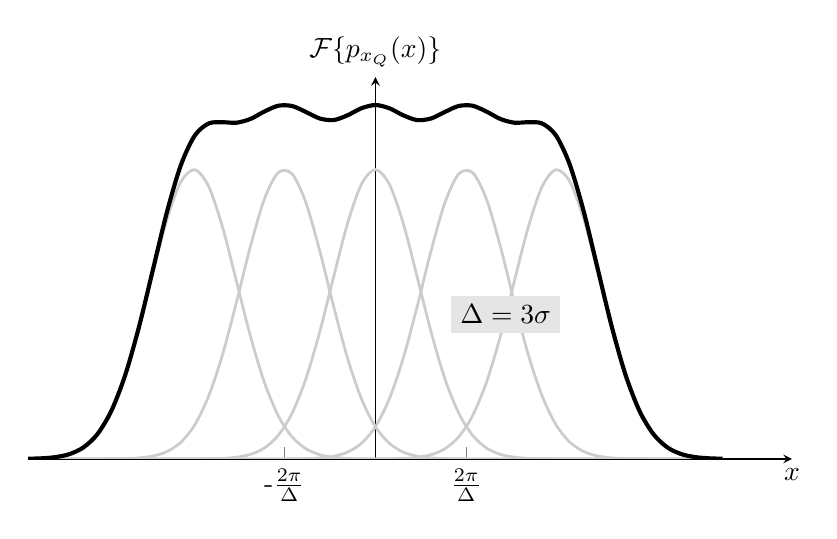
\begin{tikzpicture}
\begin{axis}[
	axis lines*=middle,
	enlargelimits = upper, clip=true,
	scale only axis,
	width=0.8\textwidth,
	height=0.4\textwidth,
	ymin=0, ymax=1.2,
	xmin=-8, xmax=8,
	axis line style={->,>=stealth},
	xlabel={$x$},
	ylabel={$\mathcal{F}\{p_{x_Q}(x)\}$},
	every axis x label/.style={
		at={(ticklabel* cs:1)},
		anchor=north,
	},
	every axis y label/.style={
		at={(ticklabel* cs:1)},
		anchor=south,
	},
	xtick={-\ws,\ws},
	xticklabels={-$\frac{2\pi}{\Delta}$, $\frac{2\pi}{\Delta}$},
	ytick=\empty,
	every outer y axis line/.append style={white!15!black},
	every y tick label/.append style={font=\color{white!15!black}},
	legend style={draw=white!15!black,fill=white,legend cell align=left}]
	\addplot [smooth, black!20, line width=1pt, domain=-8:8, samples=51] {exp(-1/2*(\sig^2*x^2))};
	\addplot [smooth, black!20, line width=1pt, domain=-8:8, samples=51] {exp(-1/2*(\sig^2*(x-\ws)^2))};
	\addplot [smooth, black!20, line width=1pt, domain=-8:8, samples=51] {exp(-1/2*(\sig^2*(x+\ws)^2))};
	\addplot [smooth, black!20, line width=1pt, domain=-8:8, samples=51] {exp(-1/2*(\sig^2*(x-2*\ws)^2))};
	\addplot [smooth, black!20, line width=1pt, domain=-8:8, samples=51] {exp(-1/2*(\sig^2*(x+2*\ws)^2))};
	\addplot [smooth, black, line width=1.5pt, domain=-8:8, samples=51] {exp(-1/2*(\sig^2*(x+2*\ws)^2)) + exp(-1/2*(\sig^2*(x+\ws)^2)) + exp(-1/2*(\sig^2*x^2)) + exp(-1/2*(\sig^2*(x-\ws)^2)) + exp(-1/2*(\sig^2*(x-2*\ws)^2))};
	\node[fill=black!10] at (axis cs: 3, 0.5) {\cap};
\end{axis}	
\end{tikzpicture}